\section{Materials and methods}

\subsection{Materials}

Table \ref{tab:materials} summarizes the materials used in this experiment. Figures \ref{fig:cannabis_skywalker-haze} and \ref{fig:cannabis_frisian-dew} show the cannabis cultivars used in this experiment, figure \ref{fig:planting-containers} the planting containers, and figures \ref{fig:led_grow_light} and \ref{fig:uv_grow_light} the LED and UV grow lights. Figure \ref{fig:spectra_uv_and_ctrl} shows the light spectra of the experimental setups with LED grow lights only (control) and with additional UV fluorescent tubes, measured with the THORLABS CCS200/M light spectrometer.

\begin{table}[htbp]
    \caption{Summary of materials used in the experiment}
    \label{tab:materials}
    \begin{tabularx}{\linewidth}{l|X}
        \toprule
        \textbf{Item} & \textbf{Description} \\
        \midrule
        Seeds\index{seeds!cannabis} & 2 seeds of DUTCH PASSION Skywalker Haze\index{seeds!cannabis!Skywalker Haze} (feminized) \\
        & 10 seeds of DUTCH PASSION Frisian Dew seeds\index{seeds!cannabis!Frisian Dew} (feminized) \\
        \bigstrut
        Planting containers\index{planting container} & \qty[mode=text]{3}{\L} fabric planting containers from Chiliwelten with zipper \\
        & \qty[mode=text]{15}{\L} fabric planting containers from Chiliwelten with zipper \\
        \bigstrut
        Potting soil\index{potting soil} & Lightly fertilized organic coconut potting soil with added mycorrhizae\index{mycorrhizae} (for seeds) \\
        & Fertilized organic coconut potting soil (for potting up) \\
        \bigstrut
        LED Grow lights\index{grow light!LED} & PHLIZON FD6000 PLUS 640W Full-spectrum Daisy Chain Dimmable LED Grow Light\index{grow light!LED!PHLIZON FD6000 PLUS 640W Full-spectrum} \\
        & \quad Wattage: \qty[mode=text]{640}{\W} \\
        & \quad Color temperature/wavelengths: Full-spectrum \\
        & \quad LED distribution: \\
        & \quad \quad \num[mode=text]{1728} pcs \qtyrange[mode=text, range-phrase=\textendash, range-units=single]{2800}{3000}{\K} LEDs \\
        & \quad \quad \num[mode=text]{288} pcs \qtyrange[mode=text, range-phrase=\textendash, range-units=single]{5000}{6600}{\K} LEDs \\
        & \quad \quad \num[mode=text]{576} pcs \qtyrange[mode=text, range-phrase=\textendash, range-units=single]{660}{665}{\nm} red LEDs \\
        \bigstrut
        UV grow lights\index{grow light!UV} & LuxElite PlantUV (fluorescent tube)\index{grow light!UV!LuxElite PlantUV} \\
        & \quad Wattage: \qty[mode=text]{24}{\W} \\
        & \quad Color temperature: \qty[mode=text]{7000}{\K} \\
        & \quad UV-A: \qty[mode=text]{30}{\percent} \\
        & \quad UV-B: \qty[mode=text]{12}{\percent} \\
        \bigstrut
        Light spectrometer\index{light spectrometer} & THORLABS CCS200/M\index{light spectrometer!THORLABS CCS200/M} \\
        & \quad Wavelengths: \qtyrange[mode=text, range-phrase=\textendash, range-units=single]{200}{1000}{\nm} \\
        \bottomrule
    \end{tabularx}
\end{table}

\begin{figure}[htbp]
    \begin{subfigure}[t]{.48\textwidth}
        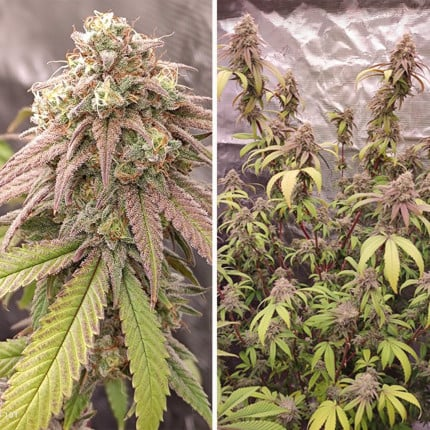
\includegraphics[width=\linewidth]{DUTCH-PASSION_Skywalker-Haze_1}
        \label{fig:cannabis_skywalker-haze_1}
    \end{subfigure}
    \begin{subfigure}[t]{.48\textwidth}
        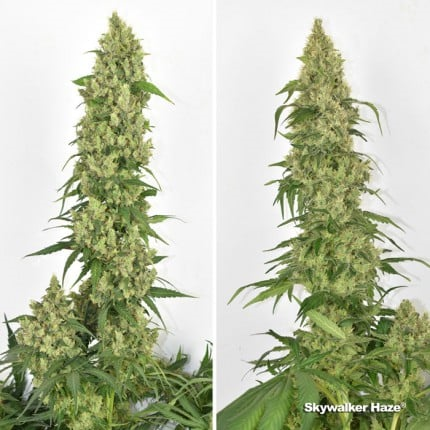
\includegraphics[width=\linewidth]{DUTCH-PASSION_Skywalker-Haze_2}
        \label{fig:cannabis_skywalker-haze_2}
    \end{subfigure}
    \caption[DUTCH PASSION Skywalker Haze]{DUTCH PASSION Skywalker Haze cultivar. From: \fullcite{noauthor_dutch-passion_skywalker-haze_nodate}}
    \label{fig:cannabis_skywalker-haze}
\end{figure}

\begin{figure}[htbp]
    \begin{subfigure}[t]{.48\textwidth}
        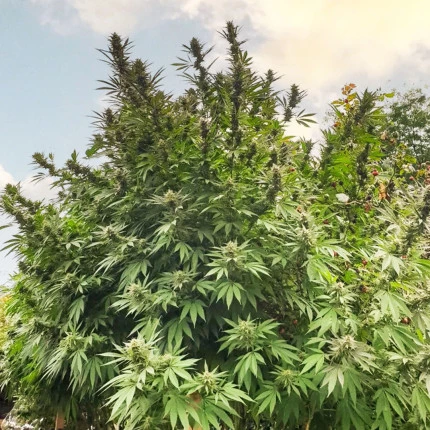
\includegraphics[width=\linewidth]{DUTCH-PASSION_Frisian-Dew_1}
        \label{fig:cannabis_frisian-dew_1}
    \end{subfigure}
    \begin{subfigure}[t]{.48\textwidth}
        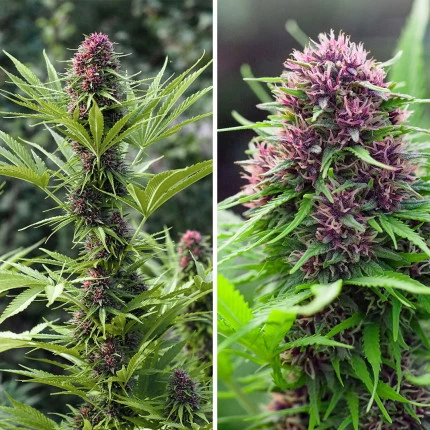
\includegraphics[width=\linewidth]{DUTCH-PASSION_Frisian-Dew_2}
        \label{fig:cannabis_frisian-dew_2}
    \end{subfigure}
    \caption[DUTCH PASSION Frisian Dew]{DUTCH PASSION Frisian Dew cultivar. From: \fullcite{noauthor_dutch-passion_frisian-dew_nodate}}
    \label{fig:cannabis_frisian-dew}
\end{figure}

\begin{figure}[htbp]
    \begin{subfigure}[t]{.48\textwidth}
        \includegraphics[width=\linewidth]{Chiliwelten_3L-Stofftopf-Reißverschluss}
        \caption{\qty[mode=text]{3}{\L} planting container. From: \fullcite{noauthor_chiliwelten_3l_nodate}}
        \label{fig:planting-container-3L}
    \end{subfigure}
    \begin{subfigure}[t]{.48\textwidth}
        \includegraphics[width=\linewidth]{Chiliwelten_15L-Stofftopf-Reißverschluss}
        \caption{\qty[mode=text]{15}{\L} planting container. From: \fullcite{noauthor_chiliwelten_15l_nodate}}
        \label{fig:planting-container-15L}
    \end{subfigure}
    \caption[Planting containers used in this experiment]{The \qty[mode=text]{3}{\L} and \qty[mode=text]{15}{\L} fabric planting containers from Chiliwelten with zipper used in this experiment}
    \label{fig:planting-containers}
\end{figure}

\begin{figure}[htbp]
    \begin{subfigure}[t]{.48\textwidth}
        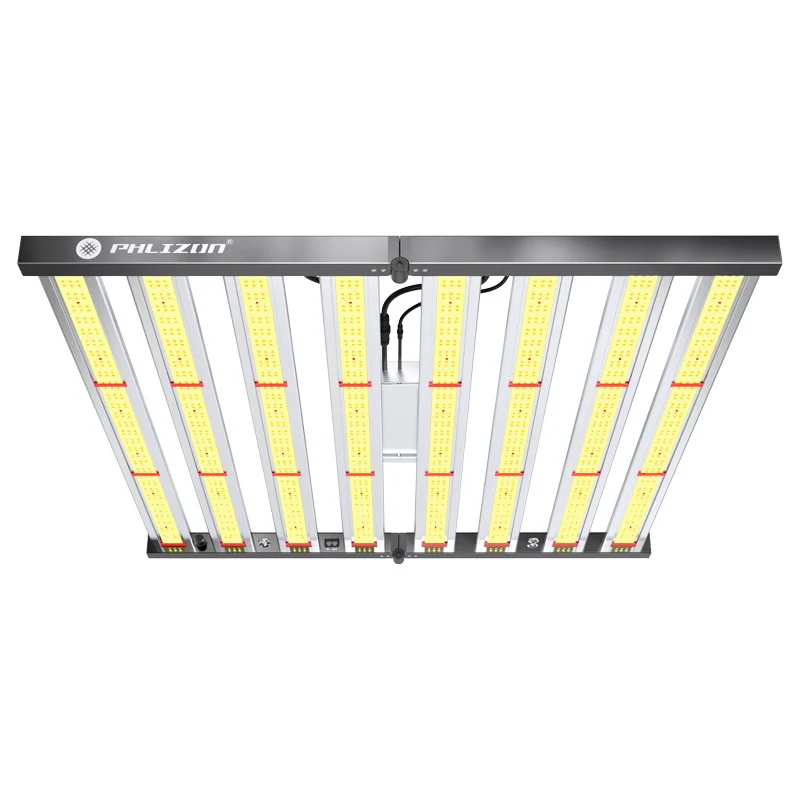
\includegraphics[width=\linewidth]{PHLIZON_PH-FD8-E}
        \label{fig:led_grow_light_img}
    \end{subfigure}
    \begin{subfigure}[t]{.48\textwidth}
        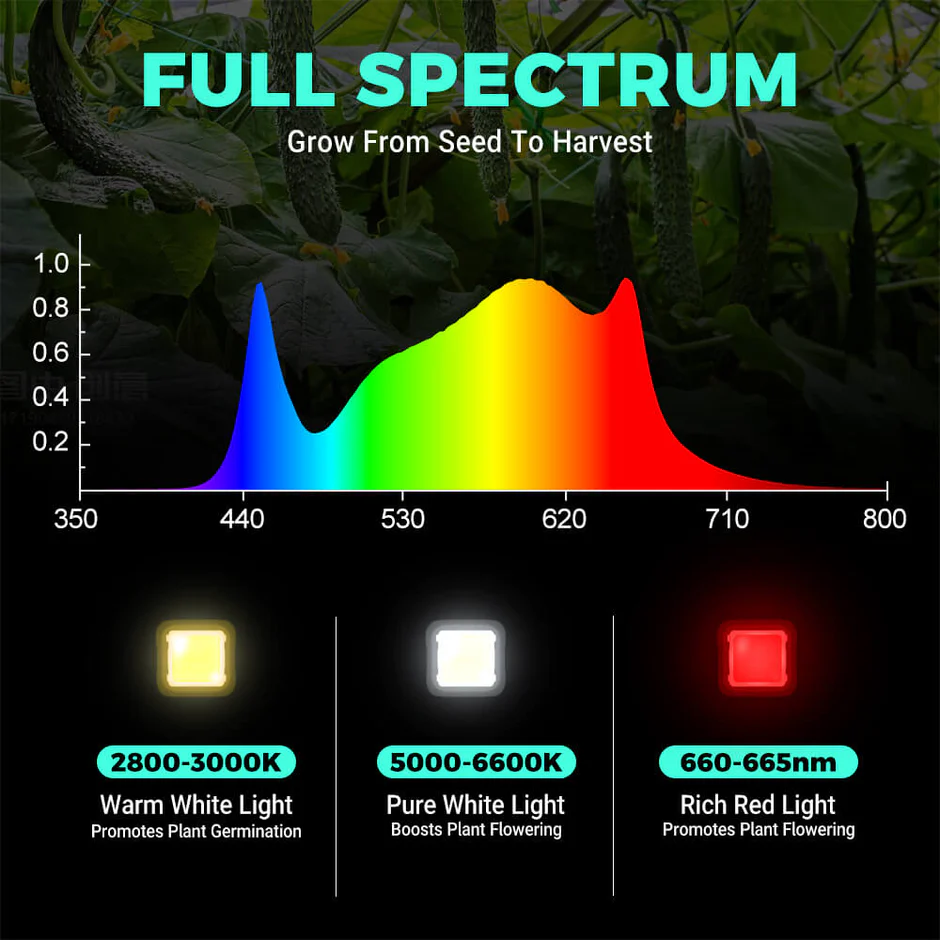
\includegraphics[width=\linewidth]{PHLIZON_PH-FD8-E_light-spectrum}
        \label{fig:led_grow_light_spectrum}
    \end{subfigure}
    \caption[LED grow light used in this experiment]{LED grow light used in this experiment. From \fullcite{noauthor_phlizon_fd6000-640w-upgraded_nodate}}
    \label{fig:led_grow_light}
\end{figure}

\begin{figure}[htbp]
    \begin{subfigure}[t]{.48\textwidth}
        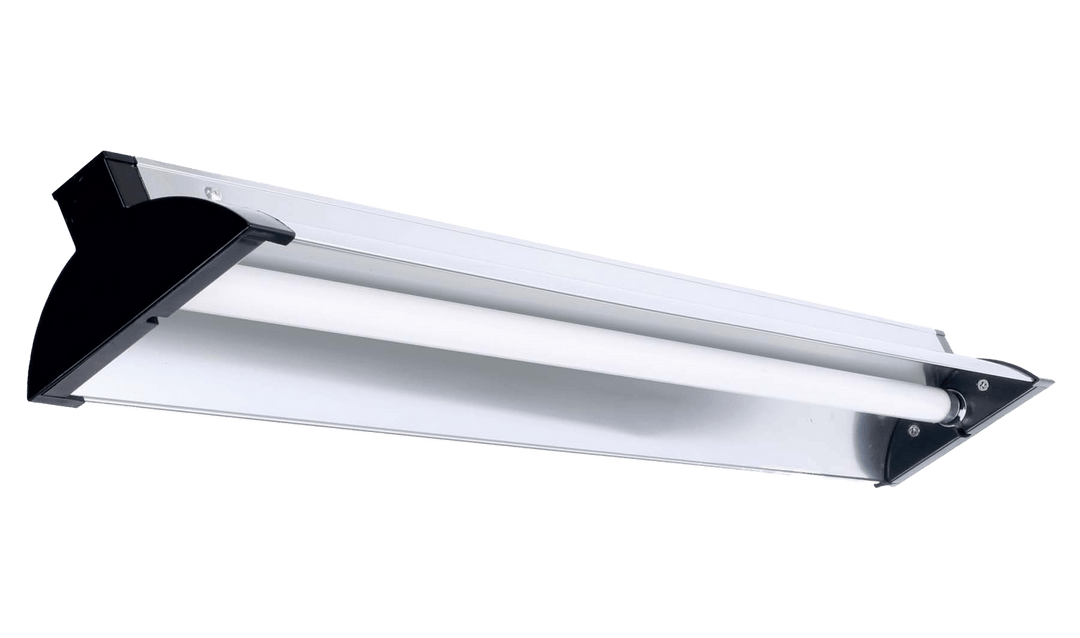
\includegraphics[width=\linewidth]{LuxElite_PlantUV}
        \label{fig:uv_grow_light_img}
    \end{subfigure}
    \begin{subfigure}[t]{.48\textwidth}
        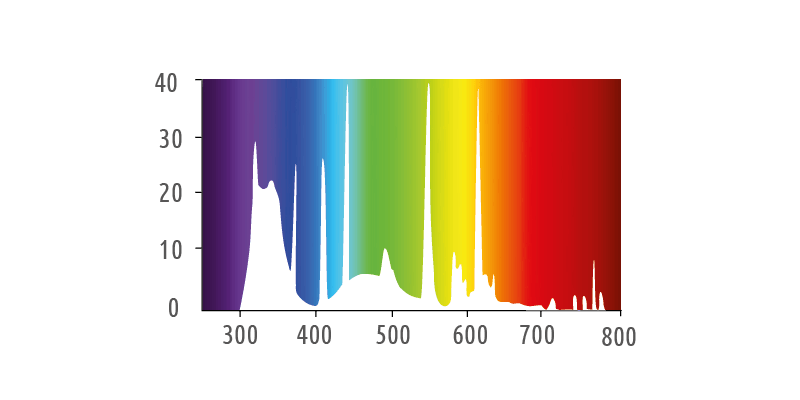
\includegraphics[width=\linewidth]{LuxElite_PlantUV_light-spectrum}
        \label{fig:uv_grow_light_spectrum}
    \end{subfigure}
    \caption[UV grow light used in this experiment]{UV grow light used in this experiment. From \fullcite{noauthor_luxelite_plantuv_nodate}}
    \label{fig:uv_grow_light}
\end{figure}

\begin{figure}[htbp]
    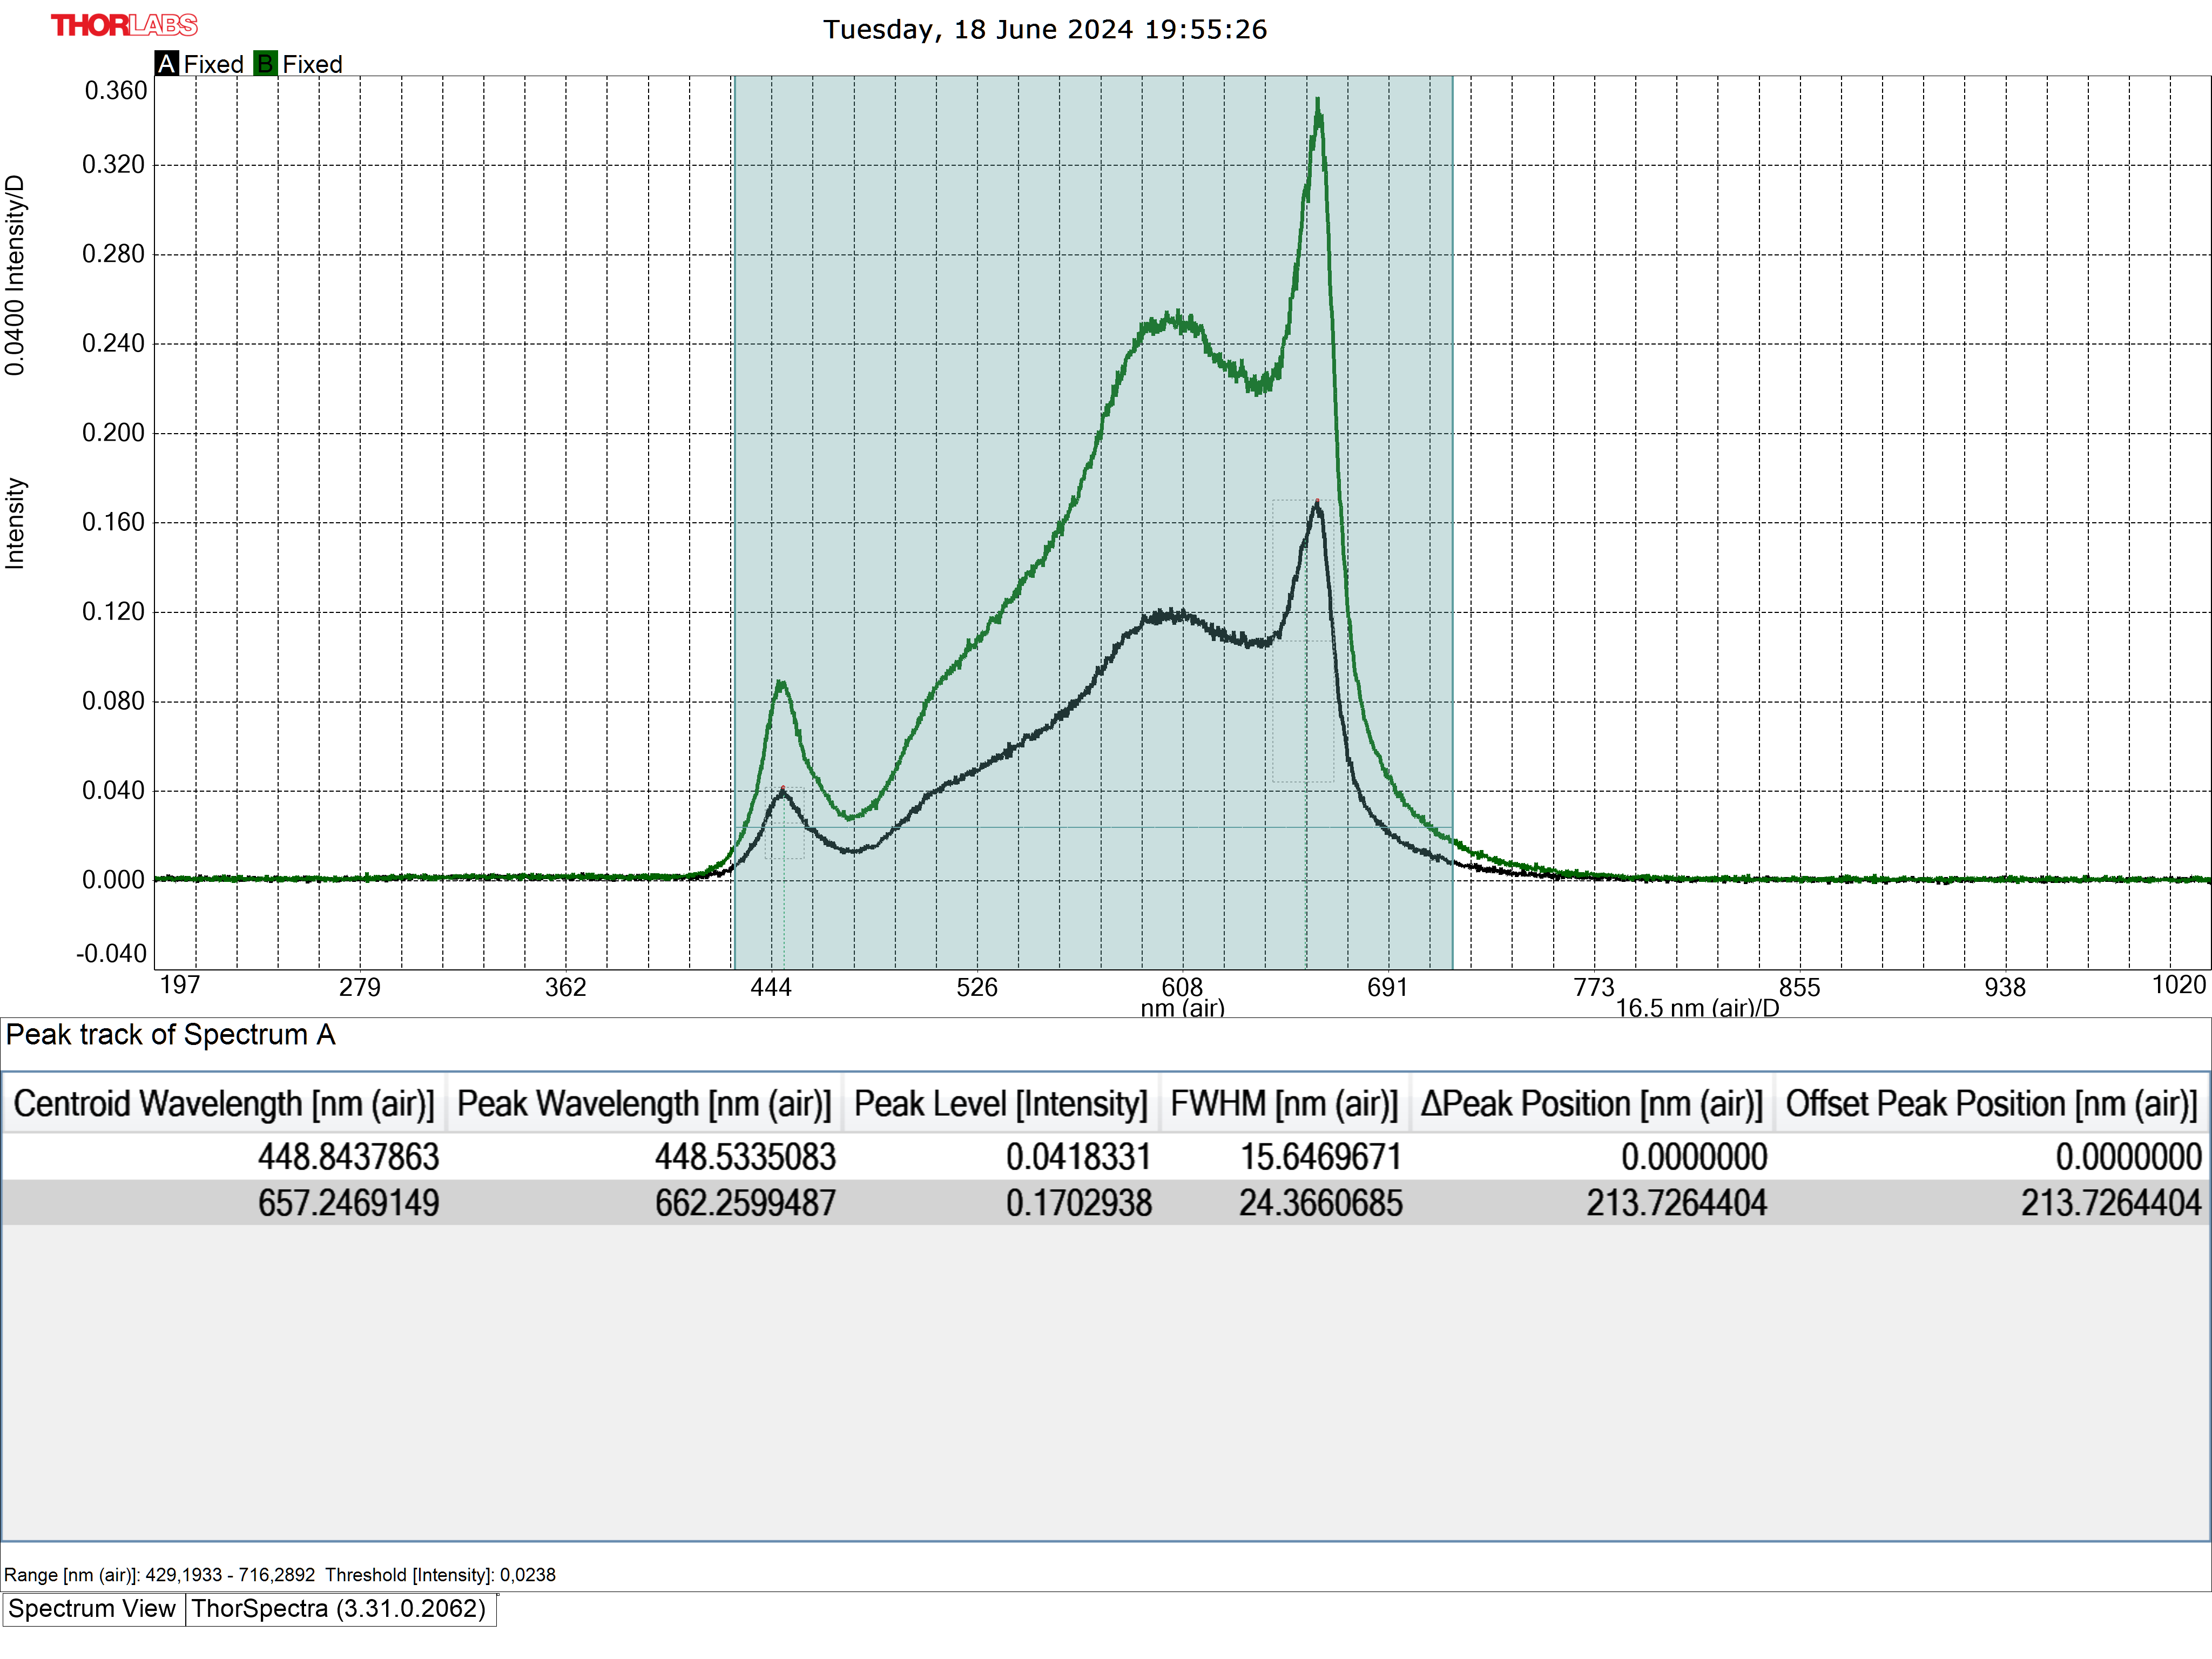
\includegraphics[width=\linewidth]{spectra_uv_and_ctrl}
    \caption[Light spectra of the experimental setups]{Light spectra of the experimental setups with LED grow lights only (control) and with additional UV fluorescent tubes, measured with the THORLABS CCS200/M light spectrometer\index{light spectrometer!THORLABS CCS200/M}. The green graph represents the spectrum of the control setup, and the black graph represents the spectrum of the UV setup. Differences in the intensities of the two graphs are due to the measurement procedure and do not indicate actual differences in light intensities. The spectra reveal that the intensities of the UV lights are negligible compared to the LED grow lights.}
    \label{fig:spectra_uv_and_ctrl}
\end{figure}

\subsection{Experimental procedure}

On May 2, two seeds of DUTCH PASSION Skywalker Haze (feminized) and ten seeds of DUTCH PASSION Frisian Dew (feminized) and  were planted in \qty[mode=text]{3}{\L} fabric planting containers filled with lightly fertilized organic coconut potting soil with added mycorrhizae. The seeds were germinated and initially grown under full-spectrum LED lights (PHLIZON FD6000 PLUS 640W). The plants were divided into two groups, with one group receiving additional light from four LuxElite PlantUV grow lights.

On May 13, these plants were transplanted into \qty[mode=text]{15}{\L} fabric planting containers with fertilized organic coconut potting soil.

On June 17, after \num[mode=text]{46} days of growth, the plants were assessed for the following growth parameters:
\begin{itemize}
    \item Plant height\index{growth parameter!plant height}: Measured from the base of the stem to the highest point using a ruler.
    \item Stem circumference\index{growth parameter!stem circumference}: Measured directly under the first stem node.
    \item Number of internodes\index{growth parameter!number of internodes}: Counted from the base to the topmost stem node.
\end{itemize}

Additionally, light conditions were measured using a THORLABS CCS200/M light spectrometer\index{light spectrometer!THORLABS CCS200/M}.

Figure \ref{fig:process_chain} outlines the sequence of experimental procedures.

\begin{figure}[htbp]
    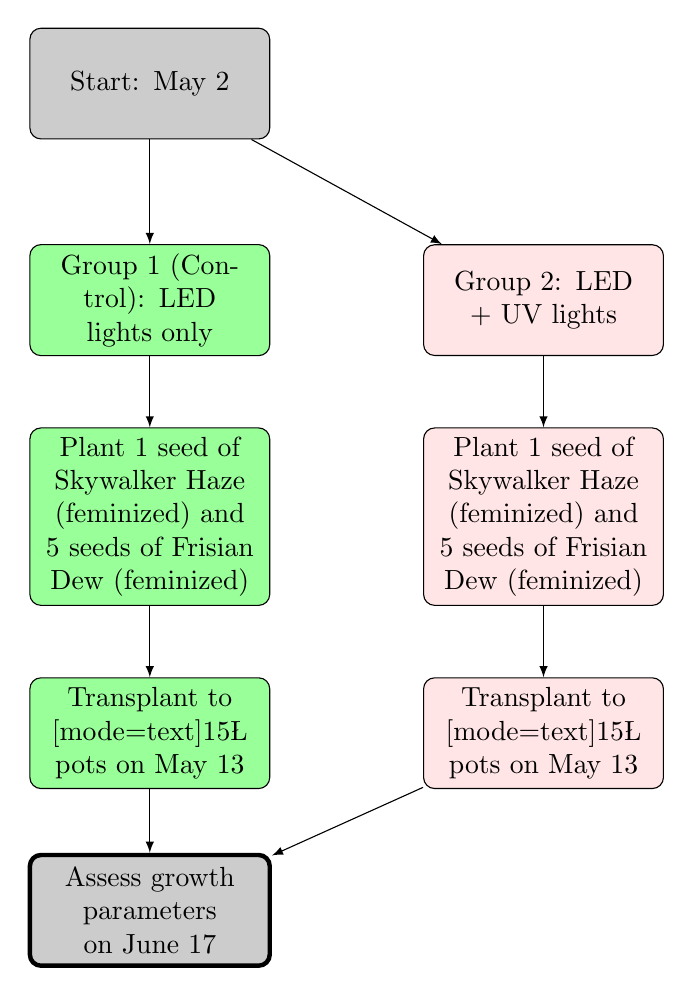
\begin{tikzpicture}[node distance=2.75cm, auto]
        % Define styles
        \tikzstyle{box_all_groups} = [rectangle, draw, fill=gray!40, text width=8em, text centered, rounded corners, minimum height=4em]
        \tikzstyle{box_ctrl_group} = [rectangle, draw, fill=green!40, text width=8em, text centered, rounded corners, minimum height=4em]
        \tikzstyle{box_exp_group} = [rectangle, draw, fill=pink!40, text width=8em, text centered, rounded corners, minimum height=4em]
        \tikzstyle{line} = [draw, -latex]

        % Nodes
        \node [box_all_groups] (start) {Start: May 2};

        \node [box_ctrl_group, below of=start, node distance=2.75cm] (ctrl_group_start) {Group 1 (Control): LED lights only};
        \node [box_exp_group, right of=ctrl_group_start, node distance=5cm] (exp_group_start) {Group 2: LED + UV lights};

        \node [box_ctrl_group, below of=ctrl_group_start, node distance=2.75cm] (ctrl_group_seed) {Plant  1 seed of Skywalker Haze (feminized) and 5 seeds of Frisian Dew (feminized)};
        \node [box_exp_group, below of=exp_group_start, node distance=2.75cm] (exp_group_seed) {Plant  1 seed of Skywalker Haze (feminized) and 5 seeds of Frisian Dew (feminized)};

        \node [box_ctrl_group, below of=ctrl_group_seed, node distance=2.75cm] (ctrl_group_transplant) {Transplant to \qty[mode=text]{15}{\L} pots on May 13};
        \node [box_exp_group, below of=exp_group_seed, node distance=2.75cm] (exp_group_transplant) {Transplant to \qty[mode=text]{15}{\L} pots on May 13};

        \node [box_all_groups, ultra thick, below of=ctrl_group_transplant, node distance=2.25cm] (assess) {Assess growth parameters on June 17};

        % Lines
        \path [line] (start) -- (ctrl_group_start);
        \path [line] (start) -- (exp_group_start);

        \path [line] (ctrl_group_start) -- (ctrl_group_seed);
        \path [line] (exp_group_start) -- (exp_group_seed);

        \path [line] (ctrl_group_seed) -- (ctrl_group_transplant);
        \path [line] (exp_group_seed) -- (exp_group_transplant);

        \path [line] (ctrl_group_transplant) -- (assess);
        \path [line] (exp_group_transplant) -- (assess);
    \end{tikzpicture}
    \caption[Sequence of experimental procedures]{Sequence of experimental procedures. Assessments include: Plant height, stem circumference, and number of internodes.}
    \label{fig:process_chain}
\end{figure}

\subsection{Growing conditions}

The temperature\index{growing condition!temperature} was maintained at about \qty[mode=text]{21}{\degreeCelsius}. The height of the grow lights\index{grow light} was adjusted to maintain a distance of approximately \qty[mode=text]{20}{\cm} from the tip of the tallest plant. The LED grow lights\index{grow light!LED} were set to \qty[mode=text]{100}{\percent} dimmable intensity. All lights were on daily from 5:35 a.m. to 9:35 p.m. (\qty[mode=text]{16}{hr} daily). On June 17, the local sunrise was at 5:18 a.m. and the sunset was at 9:52 p.m.